  \begin{tabular}{l l l l}
    \fbox{{\bb}-1}
    &
    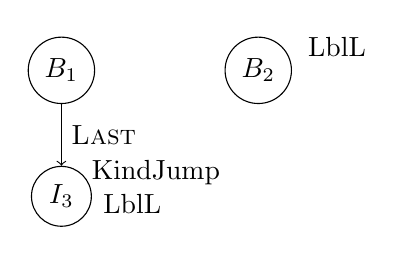
\begin{tikzpicture}[baseline]
      \node [draw,circle] (1) {$B_1$};
      \node [draw,circle,below of=1,yshift=-0.6cm] (3) {$I_3$};
      \node [right of=3,yshift=2ex,xshift=2mm] (33) {\earsattr{Kind}{Jump}};
      \node [below of=33,yshift=4ex,xshift=-3mm] (34) {\earsattr{Lbl}{L}};
      \node [draw,circle,right of=1,xshift=1.5cm] (2) {$B_2$};
      \node [right of=2,yshift=2ex] (22) {\earsattr{Lbl}{L}};

      \draw[->] (1) -- node[right] {\textsc{Last}} (3);
    \end{tikzpicture}
    &
    \coloneq
    &
    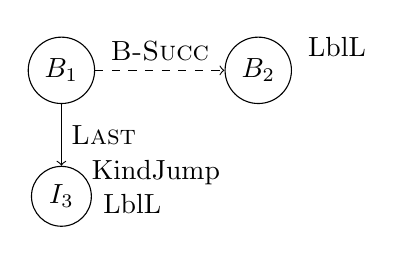
\begin{tikzpicture}[baseline]
      \node [draw,circle] (1) {$B_1$};
      \node [draw,circle,below of=1,yshift=-0.6cm] (3) {$I_3$};
      \node [right of=3,yshift=2ex,xshift=2mm] (33) {\earsattr{Kind}{Jump}};
      \node [below of=33,yshift=4ex,xshift=-3mm] (34) {\earsattr{Lbl}{L}};
      \node [draw,circle,right of=1,xshift=1.5cm] (2) {$B_2$};
      \node [right of=2,yshift=2ex] (22) {\earsattr{Lbl}{L}};

      \draw[->] (1) -- node[right] {\textsc{Last}} (3);
      \draw[->,dashed] (1) -- node[above] {\textsc{B-Succ}} (2);
    \end{tikzpicture}
  \end{tabular}

  \hdash

  \begin{tabular}{l l l l}
    \fbox{{\bb}-2}
    &
    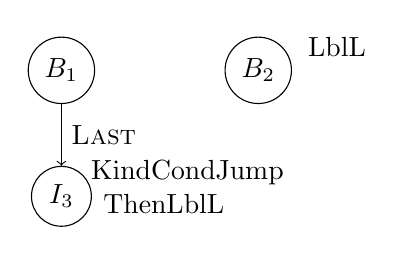
\begin{tikzpicture}[baseline]
      \node [draw,circle] (1) {$B_1$};
      \node [draw,circle,below of=1,yshift=-0.6cm] (3) {$I_3$};
      \node [right of=3,yshift=2ex,xshift=6mm] (33) {\earsattr{Kind}{CondJump}};
      \node [below of=33,yshift=4ex,xshift=-3mm] (34) {\earsattr{ThenLbl}{L}};
      \node [draw,circle,right of=1,xshift=1.5cm] (2) {$B_2$};
      \node [right of=2,yshift=2ex] (22) {\earsattr{Lbl}{L}};

      \draw[->] (1) -- node[right] {\textsc{Last}} (3);
    \end{tikzpicture}
    &
    \coloneq
    &
    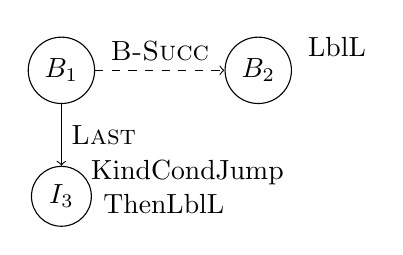
\begin{tikzpicture}[baseline]
      \node [draw,circle] (1) {$B_1$};
      \node [draw,circle,below of=1,yshift=-0.6cm] (3) {$I_3$};
      \node [right of=3,yshift=2ex,xshift=6mm] (33) {\earsattr{Kind}{CondJump}};
      \node [below of=33,yshift=4ex,xshift=-3mm] (34) {\earsattr{ThenLbl}{L}};
      \node [draw,circle,right of=1,xshift=1.5cm] (2) {$B_2$};
      \node [right of=2,yshift=2ex] (22) {\earsattr{Lbl}{L}};

      \draw[->] (1) -- node[right] {\textsc{Last}} (3);
      \draw[->,dashed] (1) -- node[above] {\textsc{B-Succ}} (2);
    \end{tikzpicture}
  \end{tabular}

  \hdash

  \begin{tabular}{l l l l}
    \fbox{{\bb}-3}
    &
    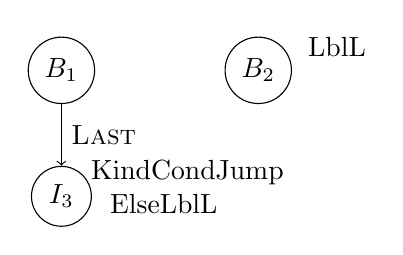
\begin{tikzpicture}[baseline]
      \node [draw,circle] (1) {$B_1$};
      \node [draw,circle,below of=1,yshift=-0.6cm] (3) {$I_3$};
      \node [right of=3,yshift=2ex,xshift=6mm] (33) {\earsattr{Kind}{CondJump}};
      \node [below of=33,yshift=4ex,xshift=-3mm] (34) {\earsattr{ElseLbl}{L}};
      \node [draw,circle,right of=1,xshift=1.5cm] (2) {$B_2$};
      \node [right of=2,yshift=2ex] (22) {\earsattr{Lbl}{L}};

      \draw[->] (1) -- node[right] {\textsc{Last}} (3);
    \end{tikzpicture}
    &
    \coloneq
    &
    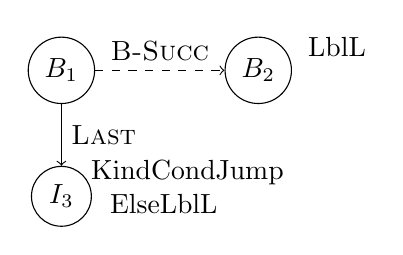
\begin{tikzpicture}[baseline]
      \node [draw,circle] (1) {$B_1$};
      \node [draw,circle,below of=1,yshift=-0.6cm] (3) {$I_3$};
      \node [right of=3,yshift=2ex,xshift=6mm] (33) {\earsattr{Kind}{CondJump}};
      \node [below of=33,yshift=4ex,xshift=-3mm] (34) {\earsattr{ElseLbl}{L}};
      \node [draw,circle,right of=1,xshift=1.5cm] (2) {$B_2$};
      \node [right of=2,yshift=2ex] (22) {\earsattr{Lbl}{L}};

      \draw[->] (1) -- node[right] {\textsc{Last}} (3);
      \draw[->,dashed] (1) -- node[above] {\textsc{B-Succ}} (2);
    \end{tikzpicture}
  \end{tabular}
